\documentclass{standalone}
\usepackage{tikz}
\usepackage{tikz-feynman} % Paquete para diagramas de Feynman
\begin{document}

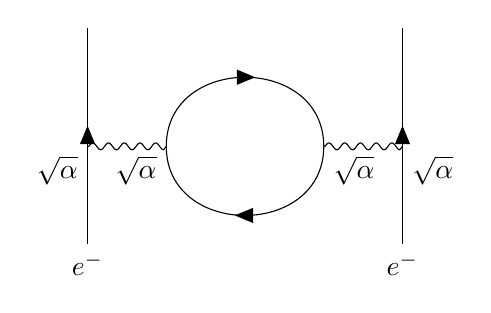
\begin{tikzpicture}
    \begin{feynman}
        % Nodos de partículas
        \vertex (e1) at (-2,-1) {$e^-$};
        \vertex (ee1) at (-2,2);
        \vertex (e2) at (2,-1) {$e^-$};
        \vertex (ee2) at (2,2);
        
        \vertex[label=below left:$\sqrt{\alpha}$] (i1) at (-2,0.5); % Fotón inicial
        \vertex [dot, label=below left:$\sqrt{\alpha}$] (v1) at (-1,0.5); % Vértice 1 con etiqueta
        \vertex [dot, label=below right:$\sqrt{\alpha}$] (v2) at (1,0.5); % Vértice 2 con etiqueta
        \vertex[label=below right:$\sqrt{\alpha}$] (f1) at (2,0.5) ; % Fotón final

        % Nodos para el bucle (par electrón-positrón)
        \vertex (looptop) at (0,0.5);
        \vertex (loopbottom) at (0,-0.5);
        
        % Diagramas de líneas
        \diagram* {
            (e1) --[fermion] (ee1), % Línea del primer electrón
            (e2) --[fermion] (ee2), % Línea del segundo electrón
            (i1) -- [photon] (v1), % Fotón virtual inicial
            (v2) -- [photon] (f1), % Fotón virtual final
            % Bucle de par electrón-positrón
            (v1) -- [fermion, half left, looseness=1.5] (v2), % Electrón
            (v2) -- [fermion, half left, looseness=1.5] (v1)  % Positrón
        };
    \end{feynman}
\end{tikzpicture}

\end{document}
